%--- 21 ----------------------------------------------------------------------------------
\item\vf{Un bon système distribué doit être plus fiable que le même système en centralisé unique.}
{\vrai}
{Un système distribué étant plus difficile à mettre en place, si celui-ci n'est pas plus fiable que son équivalent en centralisé unique alors il n'a que peu d'intérêt.


}

%--- 22 ----------------------------------------------------------------------------------
\item\vf{Dans une architecture client-serveur, on a toujours un unique serveur et un ou plusieurs clients.}
{}
{}

%--- 23 ----------------------------------------------------------------------------------
\item\vf{Une architecture de type broker peut être vue comme orientée service.}
{}
{}

%--- 24 ----------------------------------------------------------------------------------
\item\vf{Dans le cadre de services web, UDDI est un langage de description de services.}
{\faux}
{L'UDDI (\textit{\textbf{U}niversal \textbf{D}escription, \textbf{D}iscovery, and \textbf{I}ntegration}) est un annuaire de services web qui permet de les localiser sur le réseau. Il se base sur l'utilisation du langage XML pour définir la description de ces services, en reprenant quatre informations essentielles:
\begin{enumerate}
\item\textcolor{ltred}{\textsc{businessEntity}}: fournisseur
\item\textcolor{ltred}{\textsc{bussinessService}}: informations "non techniques"
\item\textcolor{ltred}{\textsc{bindingTemplate}}: informations pour accéder au service
\item\textcolor{ltred}{\textsc{tModel}}: modèle technique
\end{enumerate}
 }

%--- 25 ----------------------------------------------------------------------------------
\item\vf{Dans le cadre de services web, WSDL est un langage de description de services.}
{\vrai}
{Le WSDL (\textit{\textbf{W}eb \textbf{S}ervices \textbf{D}escription \textbf{L}anguage}) est le langage qui permet de décrire la signature précise de chaque service invoquable, c'est une grammaire XML.
\paragraph{}
Il décrit une interface d'accès à un service web qui décrit comment communiquer pour l'utiliser ("QUOI, Où, COMMENT").

\paragraph{Remarque}: XML est une grammaire soit un \textit{métalangage} (de balisage). Un tel langage permet de décrire la syntaxe (mise en forme/structure) ET la sémantique (contenu/significaiton), il s'agit donc d'une sorte de super-langage permettant la définition formelle d'autres langages de programmation.
}

%--- 26 ----------------------------------------------------------------------------------
\item\vf{Le standard REST définit les règles précises à appliquer pour obtenir des services web RESTful.}
{\vrai}
{
Une \textbf{architecture REST} est une architecture de développement web qui définit une collection de principes à respecter pour créer des service RESTful (ce n'est donc pas d'une technologie en soi).
\paragraph{}
Une \textbf{application} est dite \textbf{RESTful} si elles respectent les 6 contraintes: \textit{uniform interface, stateless, cacheable, client-server, layered system, code on demand}.
}

%--- 27 ----------------------------------------------------------------------------------
\item\vf{L’architecture d’un compilateur est typiquement orientée flux de données.}
{\vrai}
{En architecture orientée \textbf{flux} de donées, celles-ci subissent un ensemble de transformations en passant successivement par plusieurs composants indépendants. 
\paragraph{}
On retrouve principalement trois architectures de ce type:
\begin{enumerate}
\item\textcolor{ltred}{\textsc{batch séquentiel}}:
	Exécution séquentielle de sous-systèmes indépendants qui s'échangent des \textit{batchs} de données. Les transformations sont successives et chaque composant doit attendre que le précédent ait fini sont traîtement pour pouvoir commencer le sien.
	\begin{figure}[h!]
	\center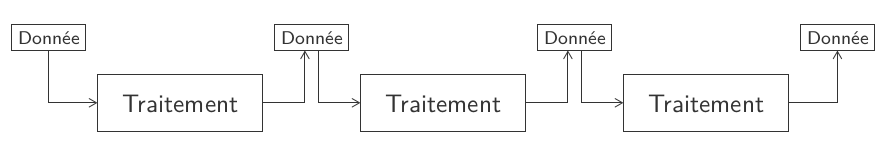
\includegraphics[scale=.3]{images/flux-donnees-batch}
	\caption{Batch séquentiel - flux de données}\cite{ref1}
	\end{figure}
	\begin{itemize}
	\paragraph{}
	\item[\textcolor{dkgreen}{\ding{52}}] Faible couplage des sous-systèmes qui n'ont connaissance que du format des données E/S. 
	\item[\textcolor{dkgreen}{\ding{52}}] Division plus simple du \textit{business data processing} en opérations élémentaires
	\end{itemize}
\item\textcolor{ltred}{\textsc{}}:
\item\textcolor{ltred}{\textsc{}}:
\end{enumerate}

}

%--- 28 ----------------------------------------------------------------------------------
\item\vf{L’architecture centrée données consiste en un data store passif et des clients actifs.}
{}
{}

%--- 29 ----------------------------------------------------------------------------------
\item\vf{L’architecture blackboard consiste en un data store passif et des clients actifs.}
{}
{}

%--- 30 ----------------------------------------------------------------------------------
\item\vf{Le cloud computing consiste simplement à installer des logiciels sur des serveurs plutôt que des
desktop stations ou laptops afin de les rendre accessibles à tout le monde via internet.}
{}
{}